\chapter{Validation} \label{chap:validation}

\section*{}

To validate the framework 3 testbeds were prepared. The first is a collection 
of small fabricated test cases where we compare the output of multiple 
simulation runs to the expected results. The second and third cases deal with 
real uses of the framework, applied in two different e-commerce contexts: the 
first is an online store of computer products and the second is a general 
comparison shopping website.

% \section{Validation methodology}

\section{Sanity checks} % rename?

\subsection{Expected number of agents in the simulation}

This test compares the number of navigation agents expected to be 
\textit{alive} at each simulation step with the actual number of them.

At each simulation step, $k$ navigation agents enter the system and  
$p_{exit}$ of them leaves, which leads to the recurrence equation \ref{eq:recc}.

\begin{equation}\label{eq:recc}
\begin{cases}
a_{1} = \left (1 - p_{exit}  \right ) k\\
a_{n} = \left (1 - p_{exit}  \right ) \left (k + a_{n - 1} \right)
\end{cases} \Leftrightarrow a_{n} = \frac{k (p_{exit}-1) ((1-p_{exit})^{n} - 
1)}{p_{exit}}
\end{equation}

The simulation run was configured in the following way:

\begin{itemize}
    \item \textbf{Website}: Sample website with 9 pages and 32 total links 
    between pages
    \item \textbf{Website agent}: Dummy agent, does not modify any page;
    \item \textbf{Navigation agent}: Sample agent implementation with a chance 
    of exiting the website of $\frac{1}{3}$ ($p_{exit}$);
    \item \textbf{Number of new navigation agents each step}: 100 ($k$)
    \item \textbf{Number of simulation steps}: 1000
\end{itemize}

Replacing the values in equation \ref{eq:recc}: $a_{n} = -200 \left ( 
\frac{2}{3}^{n} - 1 \right )$. After a few simulation runs, the expected number 
of agents in the system stabilizes: $\lim_{n\to \infty} -200 \left ( 
\frac{2}{3}^{n} - 1 \right ) = 200$.

The results of a simulation run were gathered and plotted in figure 
\ref{fig:expagents}. Triangles ($\triangle$) represent the actual value 
($A_{t}$) and circles ($\bullet$) represent the expected value ($E_{t}$) 
according to the equations above. SMAPE (symmetric mean absolute percentage 
error)\cite{makridakis1993accuracy} is used to measure the accuracy of the 
results: $ SMAPE = {\frac {1}{n}}\sum _{t=1}^{n}{\frac 
{\left|E_{t}-A_{t}\right|}{|A_{t}|+|E_{t}|}} = 3.07\% $, which is a reasonable 
low \textit{error} rate given the randomness of the system.

\begin{figure}[h]
    \begin{center}
        \leavevmode
        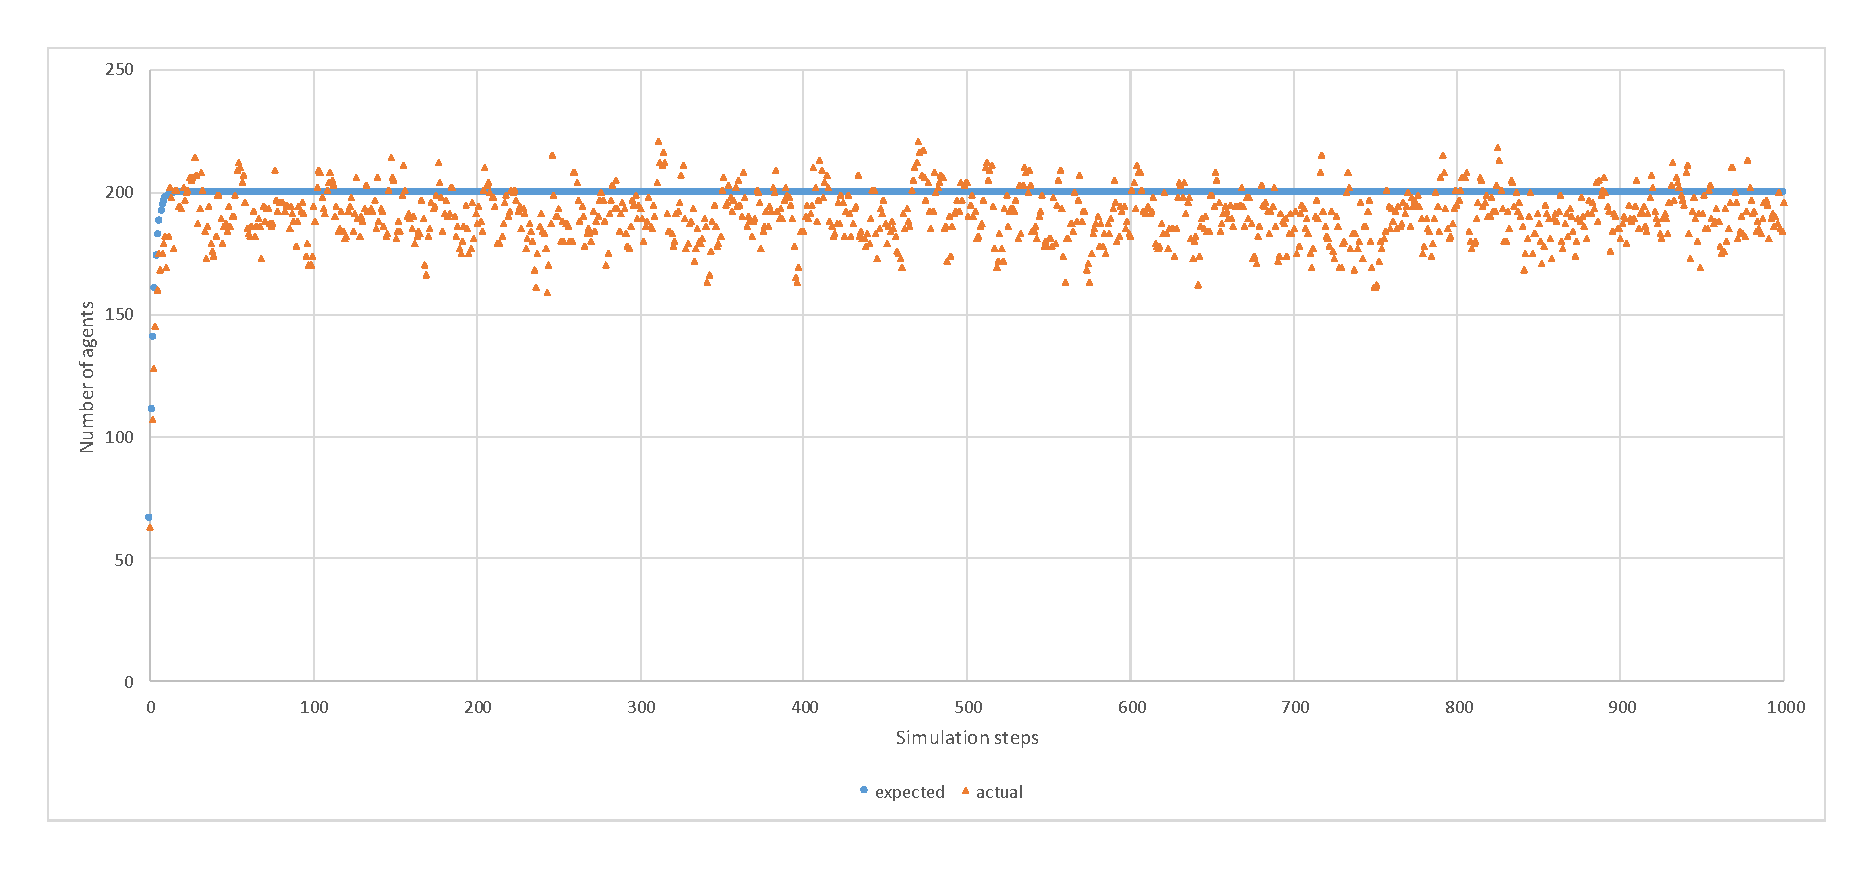
\includegraphics[width=0.95\textwidth]{expected_agents}
        \caption{Expected number of agents in the simulation}
        \label{fig:expagents}
    \end{center}
\end{figure}

\subsection{Second}

\begin{tikzpicture}
\SetGraphUnit{3}
\GraphInit[vstyle=Welsh]
\tikzset{VertexStyle/.append style = { minimum size = 24pt}}
\Vertex{page3}
\WE(page3){page2}
\WE(page2){page1}
\EA(page3){page4}
\EA(page4){page5}
\NO(page3){homepage}
\SO(page3){cart}
\tikzset{EdgeStyle/.append style = {<->}}
\Edge(homepage)(page1)
\Edge(homepage)(page2)
\Edge(homepage)(page3)
\Edge(homepage)(page4)
\Edge(homepage)(page5)
\tikzset{EdgeStyle/.append style = {->}}
\Edge(page1)(cart)
\Edge(page2)(cart)
\Edge(page3)(cart)
\Edge(page4)(cart)
\Edge(page5)(cart)
\tikzset{EdgeStyle/.append style = {->,bend left}}
\Edge(cart)(homepage)
\end{tikzpicture}

\section{Online store}

\subsection{Input data and configuration}
\subsection{Simulation}
\subsection{Results}

\section{Comparison shopping website}

\subsection{Input data and configuration}
\subsection{Simulation}
\subsection{Results}
